\documentclass{standalone}
\usepackage[utf8]{inputenc}
\usepackage{graphicx}
\usepackage{xcolor}
\usepackage{pgf,tikz}
\usepackage{mathrsfs}
\usetikzlibrary{shapes, calc, shapes, arrows, math, babel, positioning}

\begin{document}

%\tikzstyle{bag} = [text width=4em, text centered]
%\tikzstyle{end} = [circle, minimum width=3pt,fill, inner sep=0pt]
\tikzstyle{level 1} = [level distance=3.5cm, sibling distance=4cm]
\tikzstyle{level 2} = [level distance=3.5cm, sibling distance=3cm]

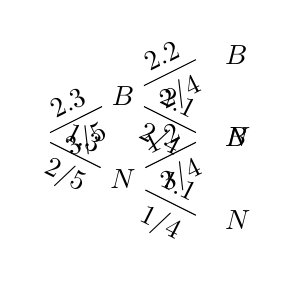
\begin{tikzpicture}[grow=right, sloped, scale=0.7]
\node[]{}
    child {
        node[]{$N$}        
            child {
                node[label=right:
                    {$N$}] {}
                edge from parent
                node[above] {$1.1$}
                node[below]  {$1/4$}
            }
            child {
                node[label=right:
                    {$B$}] {}
                edge from parent
                node[above] {$1.2$}
                node[below] {$3/4$}
            }
            edge from parent 
            node[above] {$1.3$}
            node[below]  {$2/5$}
    }
    child {
        node[]{$B$}        
        child {
                node[label=right:
                    {$N$}]{}
                edge from parent
                node[above] {$2.1$}
                node[below]  {$2/4$}
            }
            child {
                node[label=right:
                    {$B$}] {}
                edge from parent
                node[above] {$2.2$}
                node[below]  {$2/4$}
            }
        edge from parent         
            node[above] {$2.3$}
            node[below]  {$3/5$}
    };
\end{tikzpicture}




\end{document}